\newpage
\section{Realisering}
\label{realiseringOgTest}

\subsection{Hvit støy}
\label{hvitStoeoy}
For å realisere LFSRen ble det benyttet en FPGA av typen Latrice ice40, og lagd et shift register med 32 D-vipper. inngangen til den føreste D-vippen ble koblet til XOR porter som hadde inngangene koblet til utgangen av D-vippe nummer 1, 5, 6 og 31 som ambefalt av Max Maxfield \cite{LFSR}. For å iverksette LFSRen ble en knapp koblet opp til ingangen til den første D-vippen ved hjelp av en OR port. Diagramet for LFSRen kan sees i figur \ref{fig:LFSRdiagram}
% og koden kan sees i vedlegg \ref{LFSRkode}.

\begin{figure} [!h]
\centering
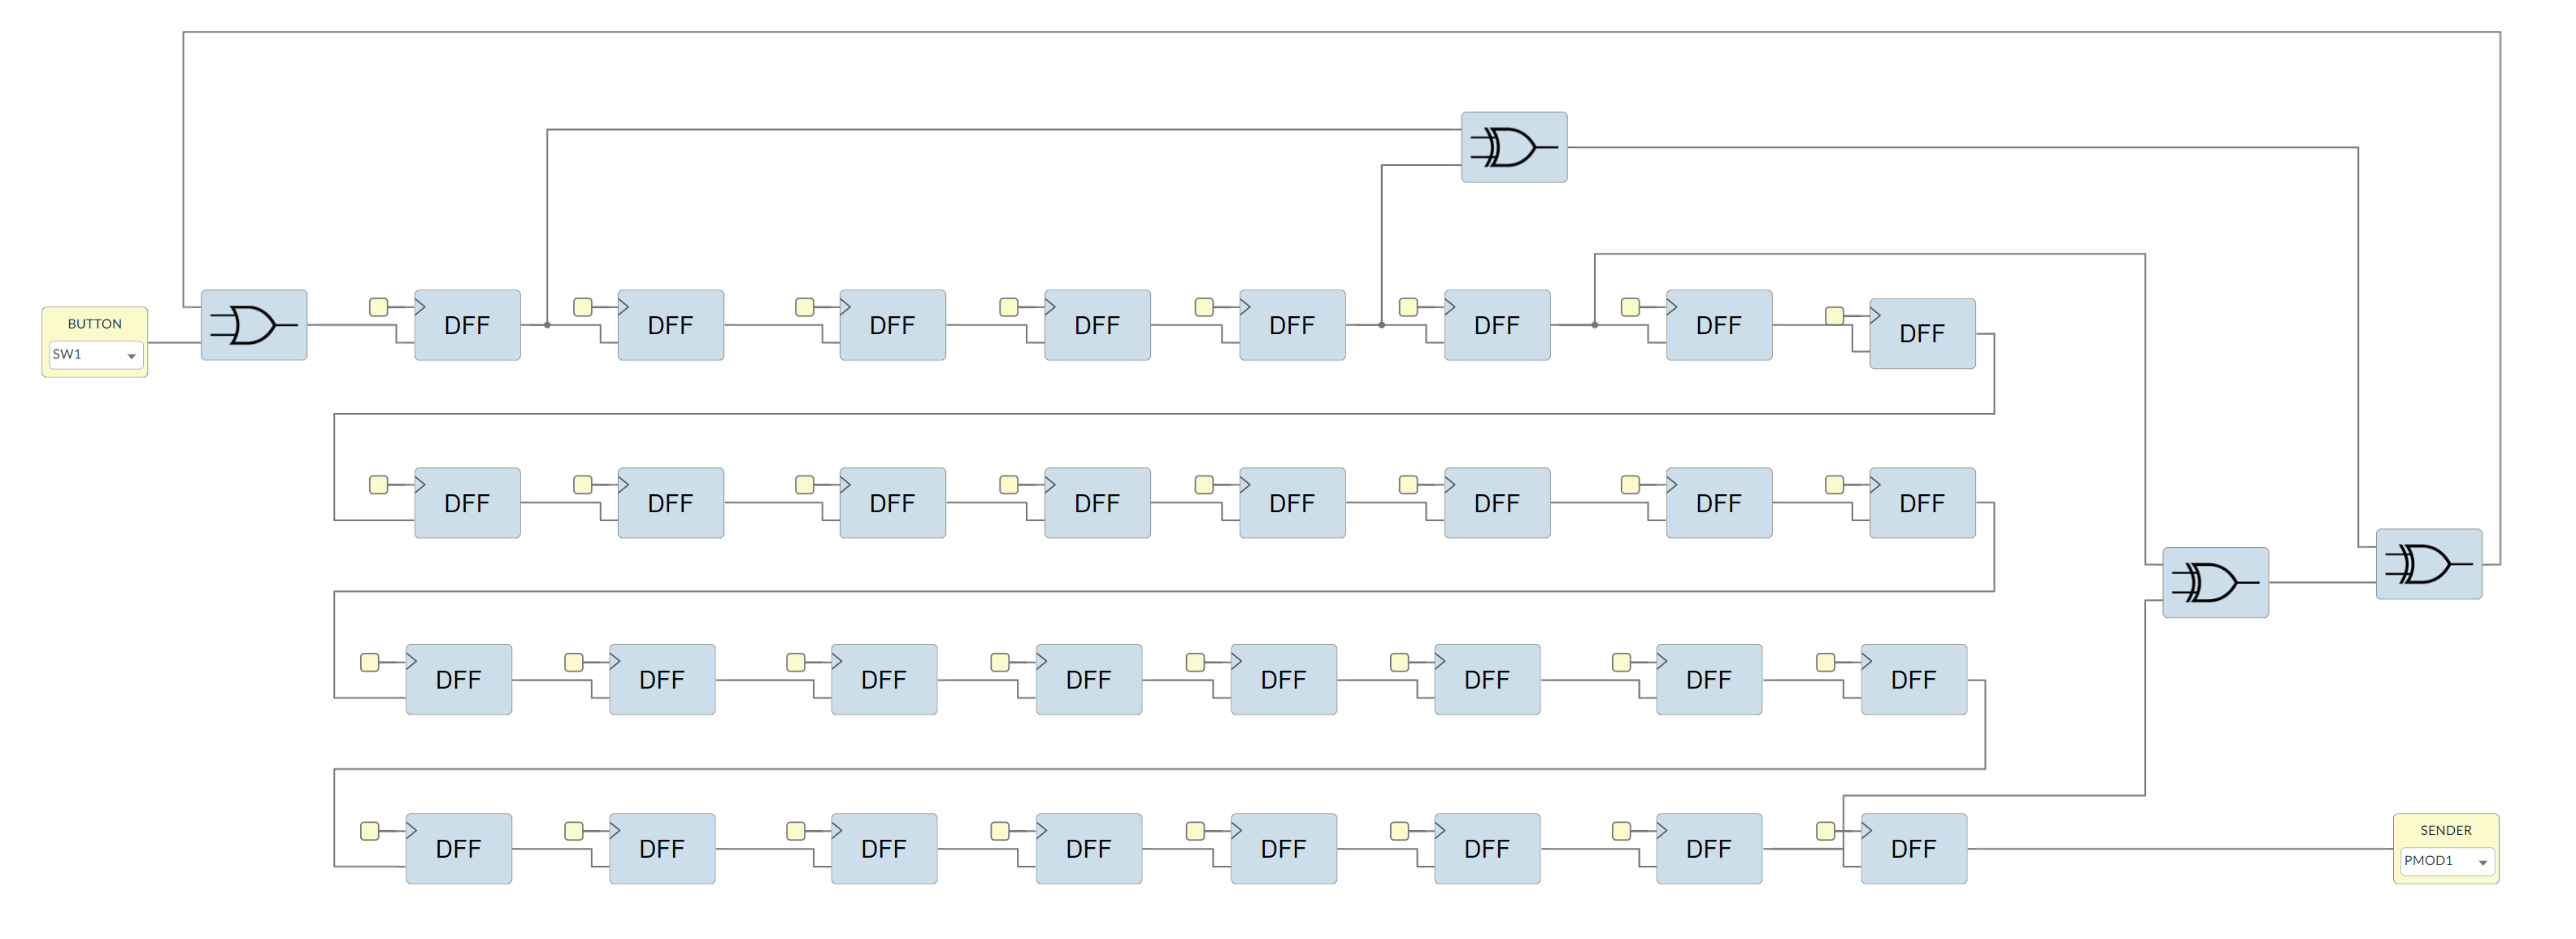
\includegraphics[width=1\linewidth]{Bilder/LFSR.png}
\caption{LFSR}
\label{fig:LFSRdiagram}
\end{figure}

\subsection{Aktivt filter}
\label{aktivtFilterRealisering}
Dette designet er tiltenkt fungere som et båndpassfilter med tiltenkt senterfrekvens på 3000Hz. Det ble regnet ut verdier ved å benytte likninge som beskrevet i \autoref{aktivtFilter} og disse verdiene ble brukt til å sette opp kretsen i figur \ref{fig:SallenKey}. Verdiene som ble benyttet kan ses i tabell \ref{tab:filterVerdier}.

\begin{table}[H]
    \centering
    \caption{Verdier for realisering av båndpassfilteret.}
    \label{tab:filterVerdier}
    \begin{tabular}{|c|c|c|c|c|c|}
    \hline
    Komponent & $R_1$ & $R_2$ & $R_3$ & $C_{1}$ & $C_{2}$ \\ \hline
    Teoretisk verdi & \SI{53}{\kilo\ohm} & \SI{266}{\Omega} & \SI{100}{\kilo\ohm} & \SI{10}{\nano\farad} & \SI{10}{\nano\farad} \\ \hline
    Realisert verdi & \SI{53}{\kilo\ohm} & \SI{240}{\Omega} & \SI{99.9}{\kilo\ohm}  & \SI{10}{\nano\farad} & \SI{10}{\nano\farad} \\ \hline
    \end{tabular}
\end{table}   
\newpage

\subsection{Test}
\label{test}
For å teste om filteret fungerete ble det først gjort en network analyse på filteret i seg selv. Dette ble gjort ved å benytte et signalgenerator og en oscilloskop. Signalet som ble generert var en sinusbølge med frekvenser fra 0 til 10kHz. Testresultatet kan ses i figur \ref{fig:filterTest}.

\begin{figure} [!h]
\centering
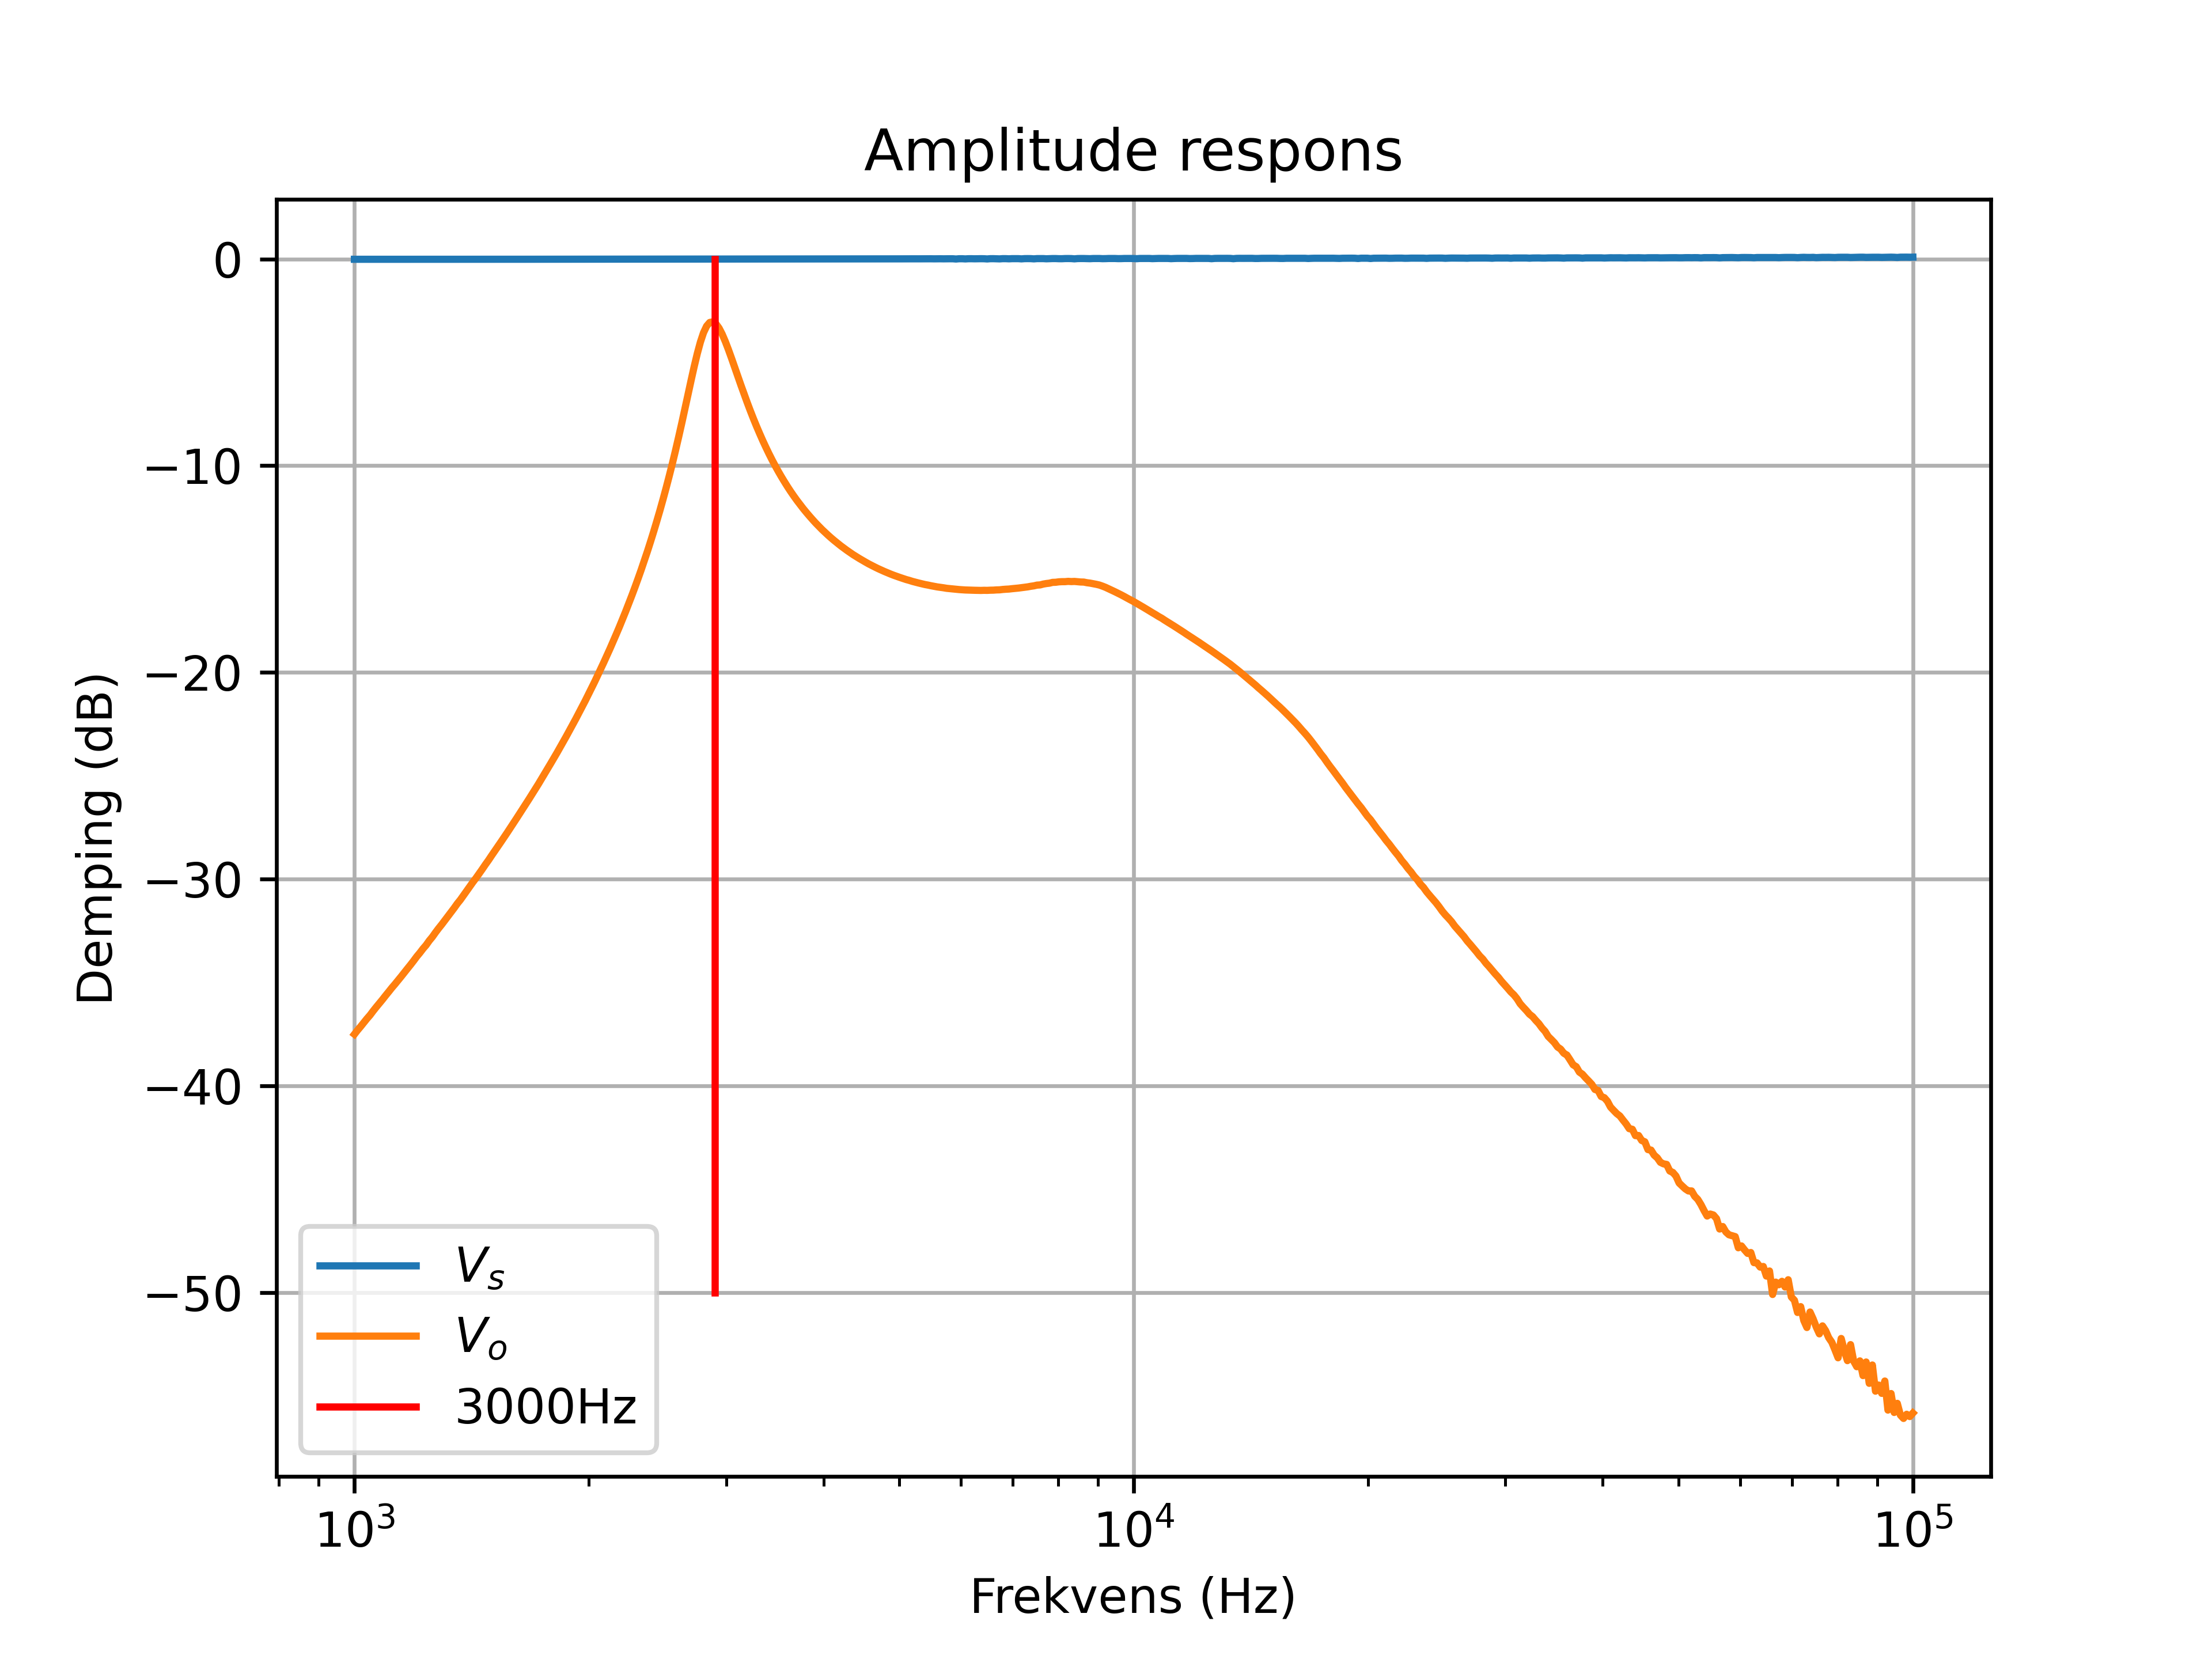
\includegraphics[width=1\linewidth]{Bilder/Network2.png}
\caption{Test av filteret}
\label{fig:filterTest}
\end{figure}

Deretter ble systemet i sin helhet testet ved å koble systemene sammen. I figur \ref{fig:systemTest} så kan man se signalet $V_s$ som er signalet som kommer ut av FPGAen og $V_{o}$ som er signalet som kommer ut av filteret. Det er tydelig at filteret fungerer som det skal og at det filtrerer bort frekvenser som ikke er i nærheten av senterfrekvensen. Amplituderesponsen til filteret slipper mest gjennom frekvenser rundt 3kHz som forventet men med en veldig redusert amplitude. Den er fremdeles hørbar uten å trenge å forsterkes hvis den spilles av direkte fra WaveForms \cite[Digilent Inc.]{Ocili}. Det var også hørbart med støy i bakrunnen som forventet, for å ungå dette kunne man brukt et høyere ordens filter og forsterket signalet etter filteret.



\begin{figure} [!h]
\centering
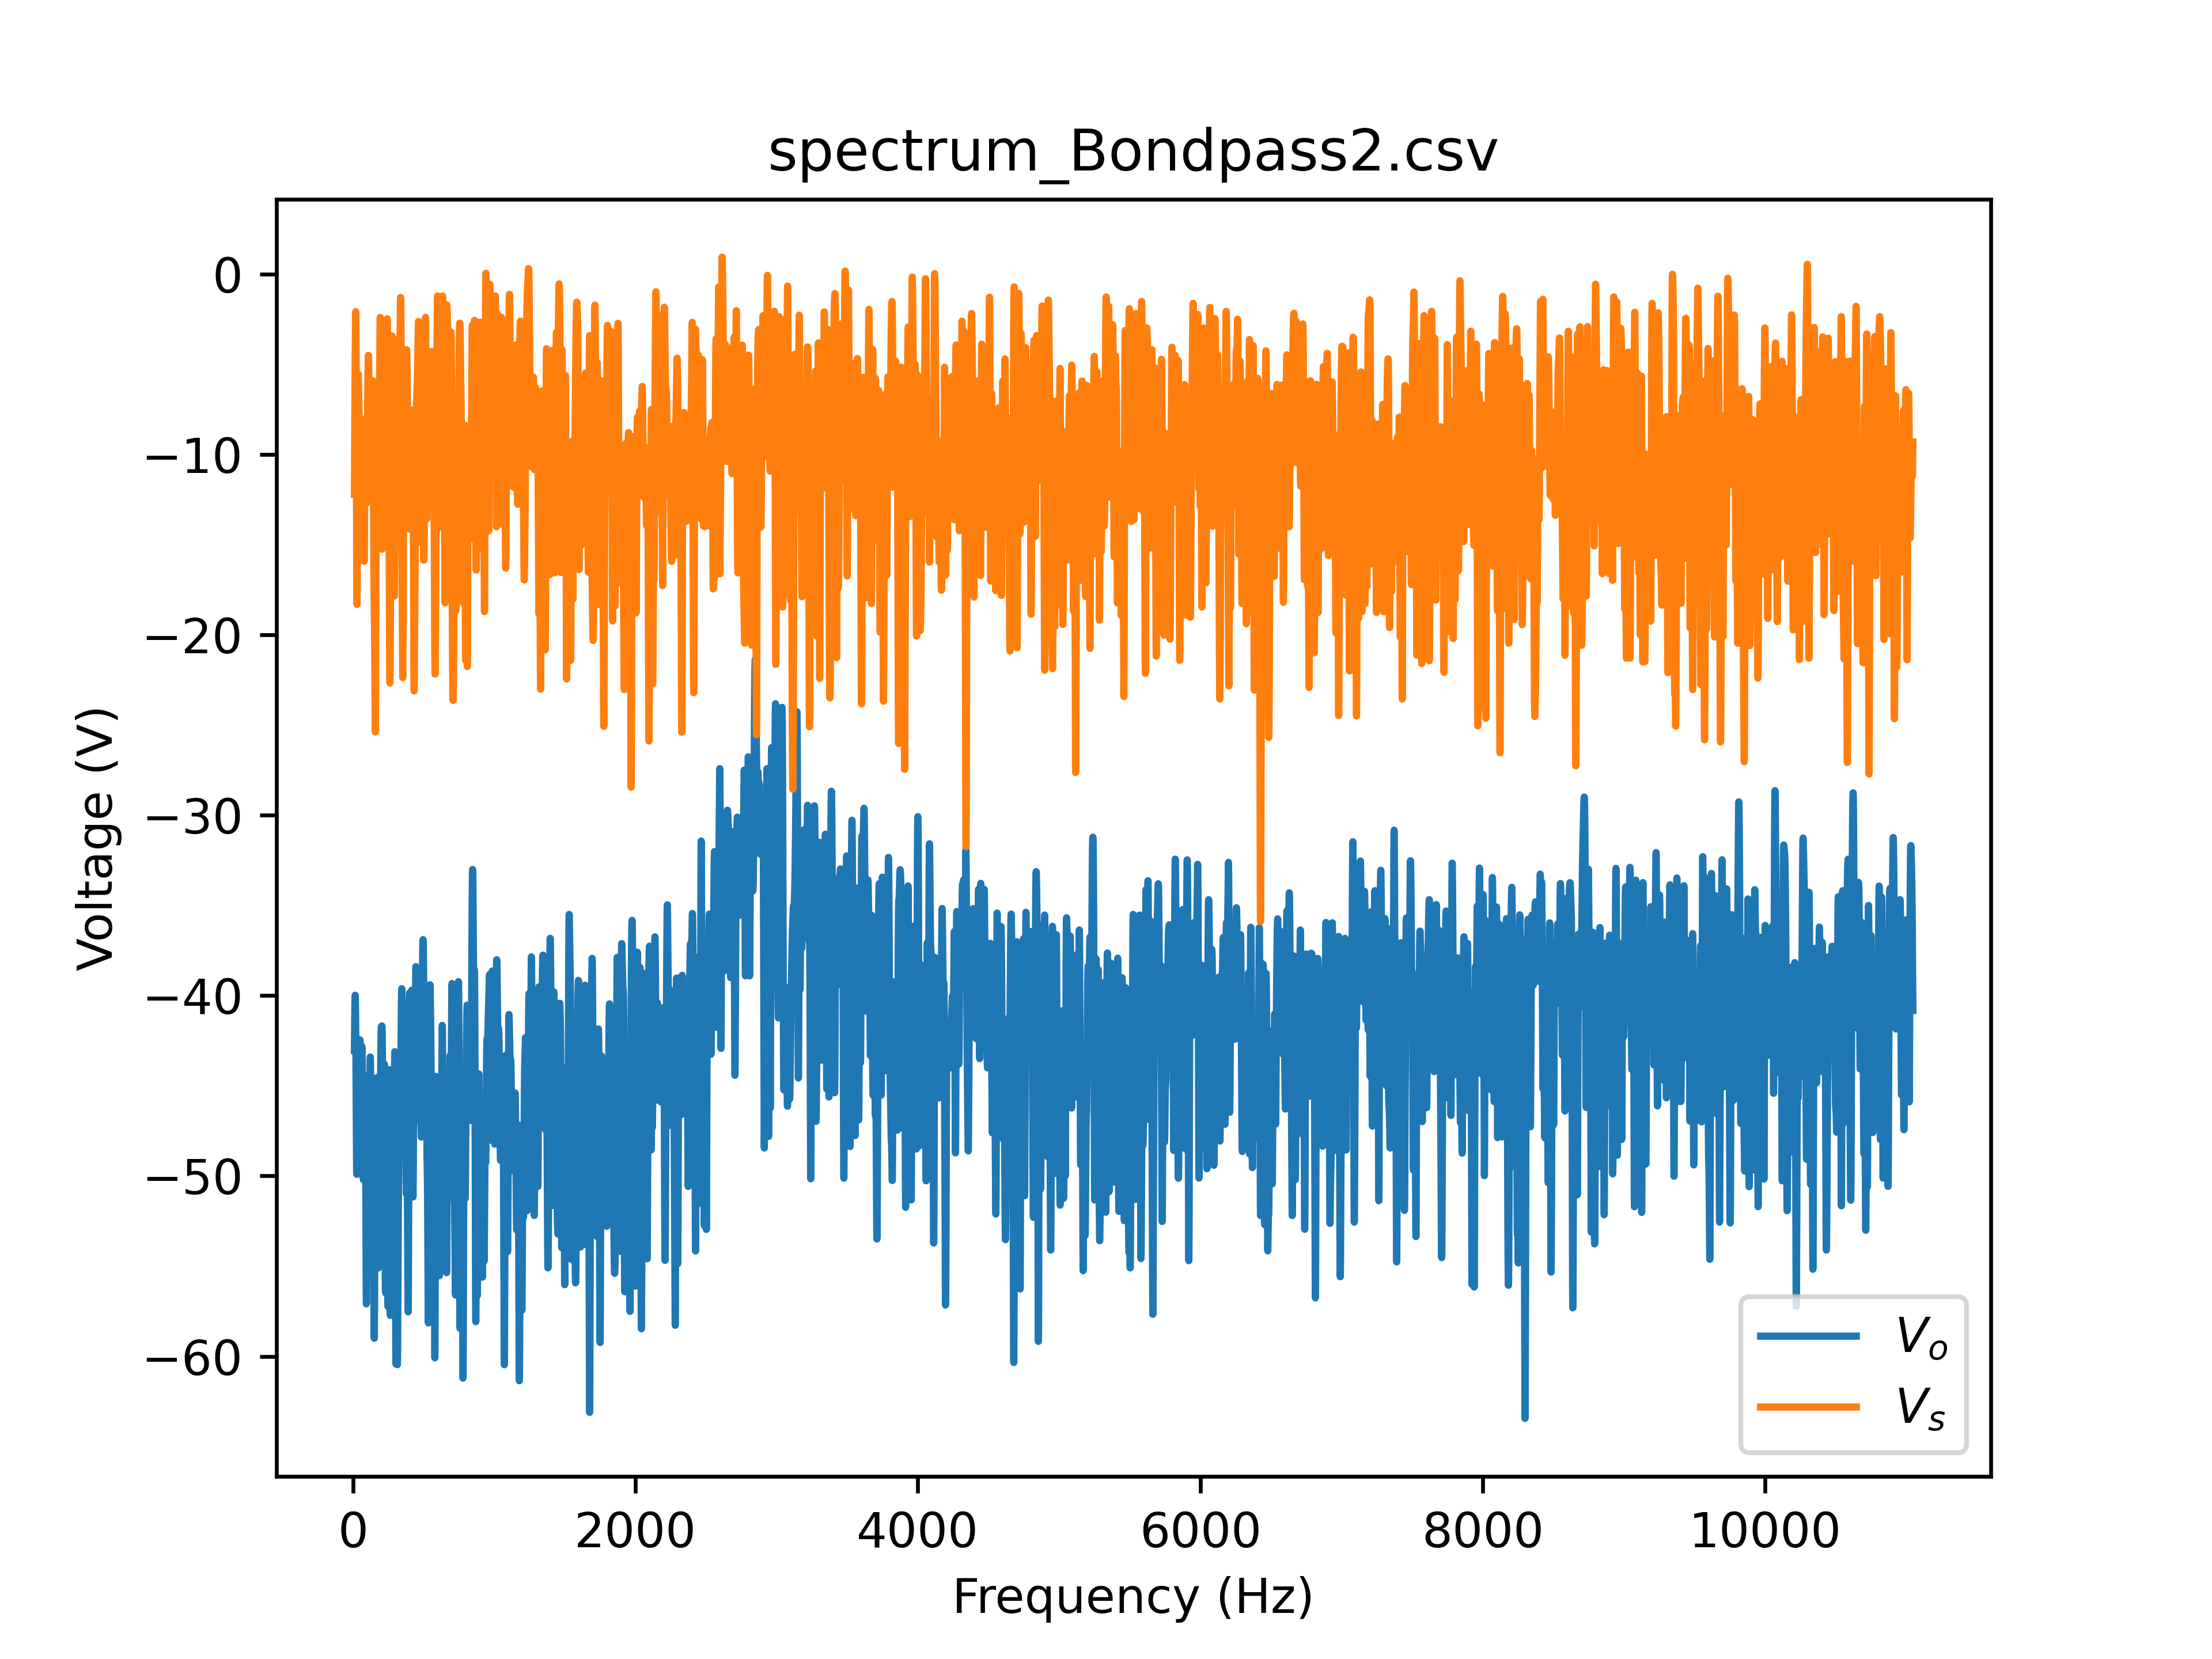
\includegraphics[width=0.8\linewidth]{Bilder/spectrum_Bondpass2.png}
\caption{Test av systemet}
\label{fig:systemTest}
\end{figure}

Et bilde som viser oppkoblet krets kan ses i figur \ref{fig:oppkobling}.

\begin{figure} [!h]
\centering
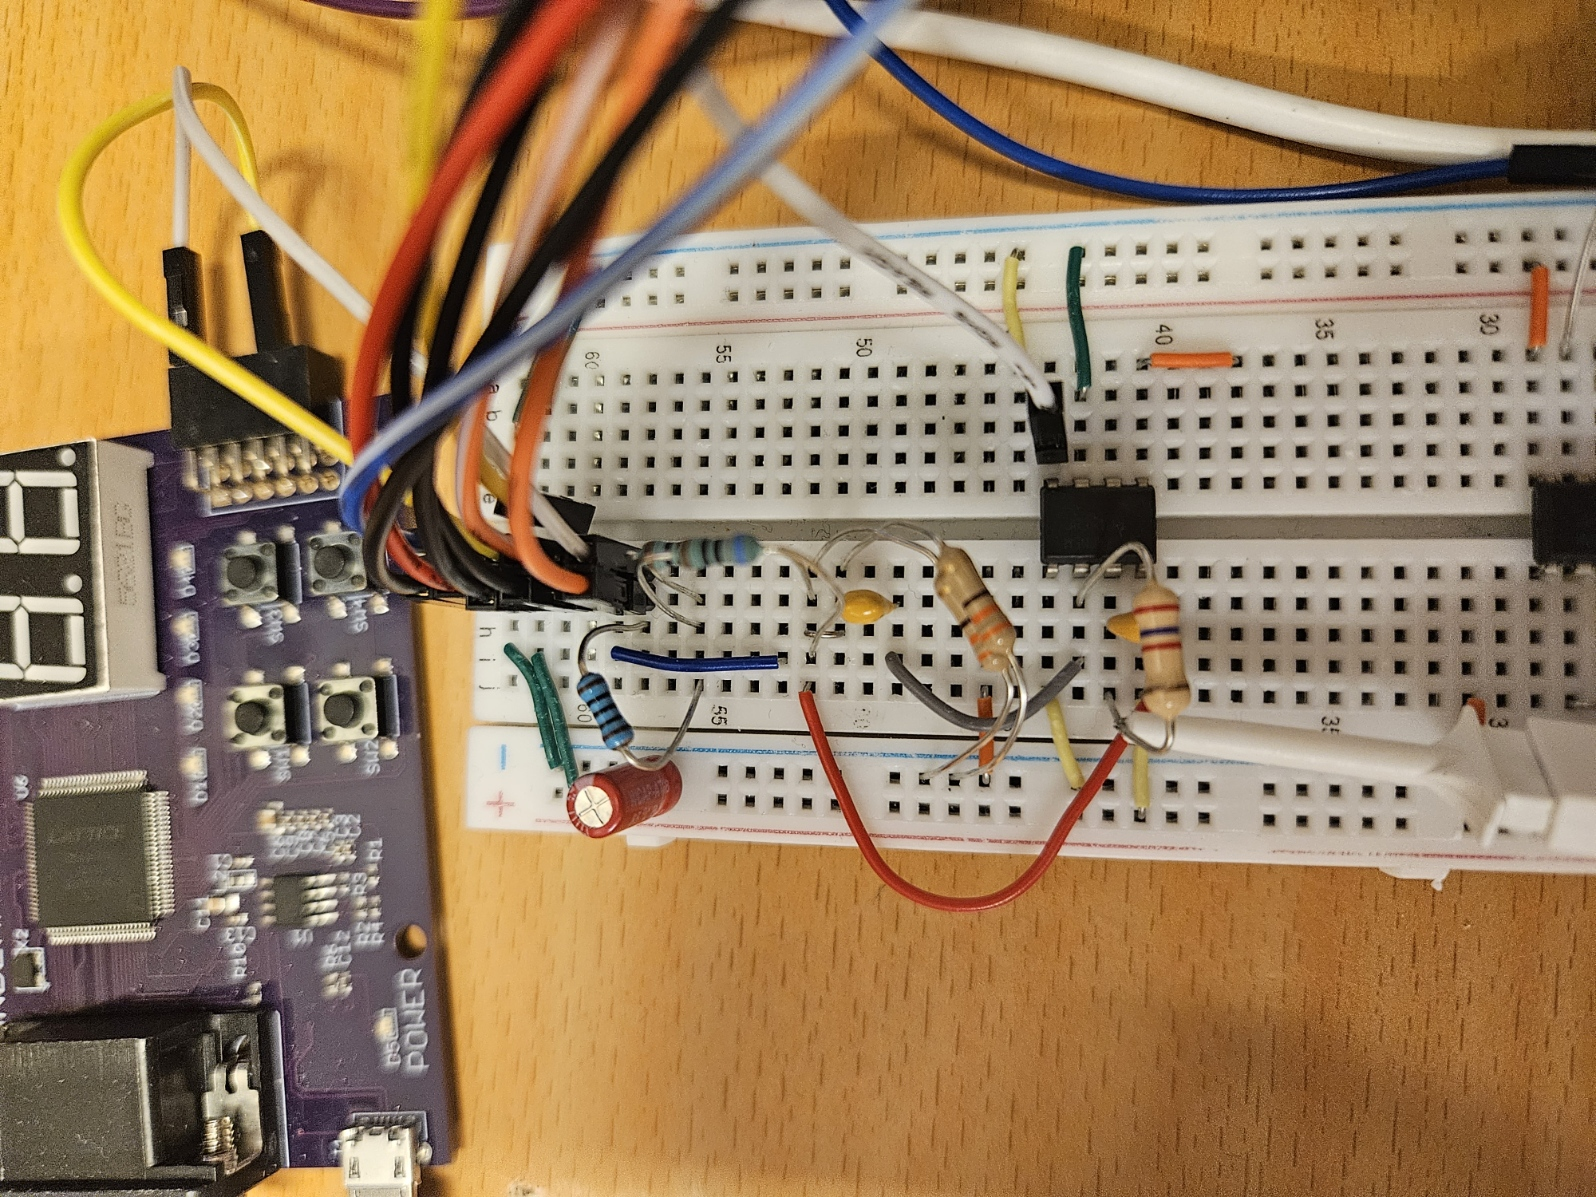
\includegraphics[width=0.6\linewidth]{Bilder/oppkobling.jpg}
\caption{Oppkobling av krets}
\label{fig:oppkobling}
\end{figure}
